\approachshort{} is implemented as a collection of programs targetting the Netronome \gls{acr:nfp} family of SmartNICs, using a mixture of the proprietary Micro-C language and P4.
As this work's implementation relies upon a good amount of platform-specific intrinsics and optimisations, it is necessary to explain some of the \gls{acr:nfp}'s basic architectural details.
These \gls{acr:soc} devices achieve scalable packet processing through sheer parallelism.
Most of the chip is composed of \glspl{acr:me}---physical cores---grouped into \emph{islands} of 4 or 12 \glspl{acr:me}.
All 12-\gls{acr:me} islands are used by a default P4 pipeline, while two of the 4-\gls{acr:me} islands are left free for user code.
Each \gls{acr:me} has \numrange{4}{8} \emph{contexts} (hardware threads) which share a code store.
%Contexts and MEs may send one another numbered signals, and MEs have a small \emph{next-neighbour} register file for passing values in one direction to the next ME on the same island.
%MEs run a proprietary instruction set, compiled to via a \emph{(Micro-)C} compiler.
Beyond registers, the platform implements an explicit memory hierarchy scaling in size, location, and access cost:
$$\text{LMEM (ME)} < \text{CLS (Island)} < \text{CTM} < \text{IMEM (Chip)} < \text{EMEM}$$
Interested readers will find more in-depth detail presented in \cref{adx:nfp-arch}.

This section covers how policy data is stored in \approachshort{} to make best use of the above memory hierarchy (\cref{sec:policy-storage}), and how cores and other resources are applied to implement both parallelism strategies described above (\cref{sec:action-and-update-computation}).
I further detail how \approachshort{} implements the \inring{} and \outring{} rings on \gls{acr:nfp} hardware (\cref{sec:agent-environment-communication}).
Through \cref{sec:intra-agent-communication}, I discuss and introduce the design of efficient work-passing and aggregation mechanisms on \gls{acr:nfp} hardware required to enable the \emph{ParSa} algorithm.
\Cref{sec:reconfigurability} describes how \approachshort{} may be configured at compile time and during runtime.
%\Cref{sec:reconfigurability} describes how \approachshort{} may be configured at compile time and during runtime, as well as presenting its control plane protocol.
Finally, I detail the scheduler used to partition tile coding tasks between available worker threads in \cref{sec:work-allocation}.


\subsection{Policy storage}\label{sec:policy-storage}
Taking advantage of the non-uniform memory architecture in \gls{acr:nfp} hardware, \approachshort{} splits its policy across the CLS, CTM and IMEM memory regions.
This arises both from necessity, and in the pursuit of runtime performance.

Firstly, policy data is stored densely, as the nature of embedded programming means that all required memory must be statically allocated.
As such, the program must reserve enough memory at compile time to contain \emph{any policy}.
While this does not rule out sparse storage, this would introduce a lookup overhead when finding the memory address of each tile's data (as well as at-rest storage costs for, e.g., a hash table).
The price in memory has already been paid for storage of a full policy, and so a dense strategy simplifies lookup by assigning a fixed (and easily computed) array index to each tiling set.

Secondly, recalling that a worker must retrieve an action preference list for each tile, we aim to minimise the latency of each memory access as part of our overall performance goal.
Ideally, this would mean placing the entirety of the policy into CLS, but there is insufficient space to do so.\sidenote{CLS is the lowest-latency memory region which is practically usable: LMEM is dedicated mostly to program state and variables which spill from the register file, and cannot be accessed across \gls{acr:me} boundaries.}
Suppose we've chosen $k=$~\num{32} for our fixed-point format, thus each action value occupies \qty{4}{\byte}.
Given $a$ action values, $d$ dimensions in a tiling, $s$ tilings in a set, and $t$ tiles per dimension, that tiling then occupies $4asd^t$~\unit{\byte} of memory---its cost scaling exponentially with the count of input dimensions.
Consider the \emph{Instant} agent design of \cref{chap:ddos-rl}: the largest tiling set chooses $a=10$, $d=4$, $s=8$ and $t=6$, and thus requires \qty{1280}{\kibi\byte}.
This alone exceeds the \qty{64}{\kibi\byte} of CLS available per island.
Worse still, we must include enough space to store \emph{any} tiling set below the maximum parameters.
If we do not differentiate between tiling sets according to dimension count, then for \emph{Instant}'s \num{17} tilings we would require \qty{21.25}{\mebi\byte}.

The solution then is to explicitly partition the policy's storage across these memory regions according to maximum dimension count; i.e., assigning tiling sets having $d\le1$ to CLS, $d\le2$ to CTM, and $d\le4$ to IMEM.
As we cannot fit a whole multidimensional policy into CLS, this design instead maximises the proportion of the policy which is placed into smaller regions.
The above dimension limits are arbitrarily picked to match \emph{Instant}/\emph{Guarded} as before, but can be customised at compile time subject to resource limits.
This increases the proportion of accesses made to lower-latency memory.
Moreover, these memory regions are accessible to all \glspl{acr:me} on the same island, and with increased access cost for remote islands.

\paragraph{Parallels in other platforms}
This tiered division of policy regions applies to other device classes as well.
For instance, \gls{acr:fpga} devices have a similar hierarchy between \glspl{acr:lut}, block \gls{acr:ram}, \gls{acr:sram} and \gls{acr:dram}.

\subsection{Action and update computation}\label{sec:action-and-update-computation}
%\approachshort{} applies the insights of \textcite{DBLP:journals/firai/TravnikMSP18} to minimise action latency; an action is computed, sent out into the environment, and only then is the underlying policy updated.
%Using one of the below strategies chosen at compile time, a state vector is tile coded, converted into action probabilities, and an action is chosen.
%This is then written out to the environment as in \cref{sec:agent-environment-communication}.

%If online learning is enabled, \approachshort{} then checks an internal hashmap for a previous state-action pair matching the current instruction source, and if found then the policy is updated.
%Updates are computed using \emph{single-step semi-gradient Sarsa}~\cite[pp. \numrange{217}{221}]{RL2E}, though modification to support other single-step methods would be trivial.
%The new state- or tiles-action pair is then written into storage.
%\approachshort{} can be configured to automatically select values of the input state vector as keys for state and reward storage.

\begin{figure}
	\centering
	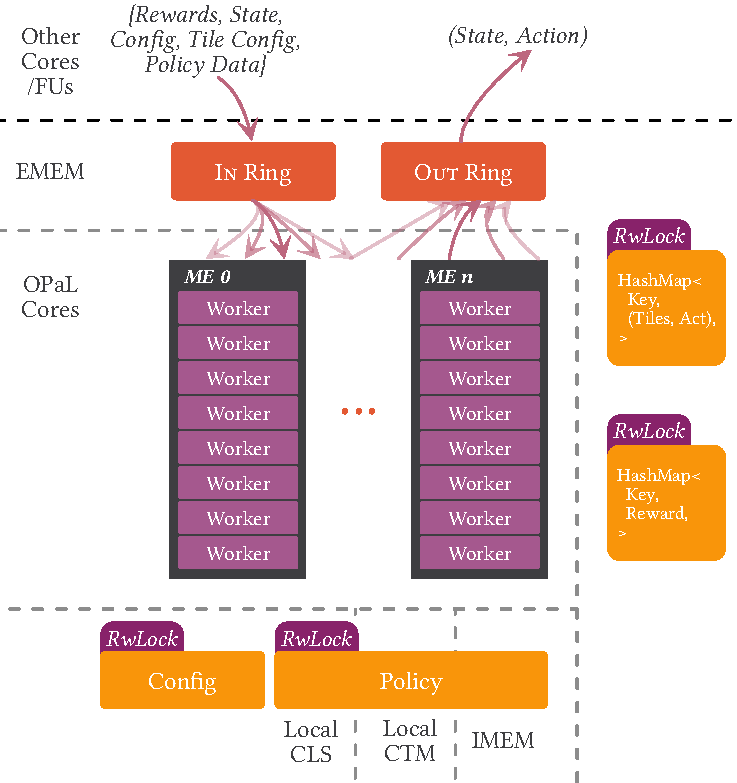
\includegraphics[keepaspectratio, width=\linewidth]{diagrams/opal/ind}
	\caption[Architectural diagram for \approachshort{}'s \Indfw{} firmware design.]{The \Indfw{} firmware design implements the first parallelism strategy discussed in \cref{sec:opal-algorithm}, where each thread \emph{independently} performs tile coded inference and Sarsa \gls{acr:rl} updates. \emph{Workers} each pull commands from (and push actions to) the environment over the \inring{} and \outring{} channels. To maintain consistency between all workers, configuration, policy data, and state-reward trajectory data must be guarded by read-write locks. During inference, workers acquire a shared read lock around, e.g., policy data. As a result, \Indfw{} optimises throughput for an \emph{offline} agent, but because policy updates require an exclusive write lock around many parameters, only a single worker may perform an \gls{acr:rl} update at any time.\label{fig:single-and-parallel:single}}
\end{figure}
\begin{figure}
	\centering
	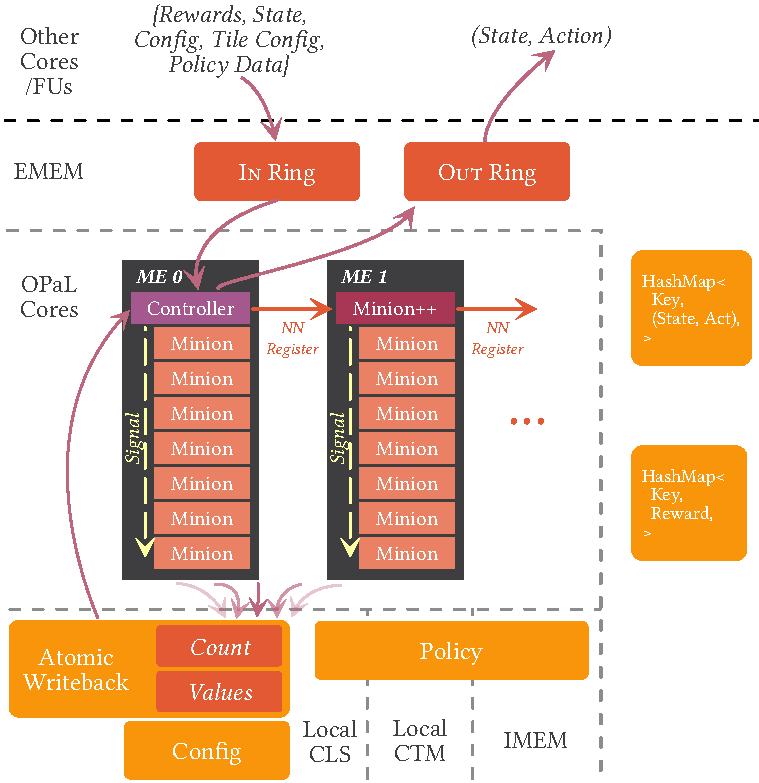
\includegraphics[keepaspectratio, width=\linewidth]{diagrams/opal/coop}
	\caption[Architectural diagram for \approachshort{}'s \Coopfw{} firmware design.]{The \Coopfw{} firmware design implements the second parallelism strategy discussed in \cref{sec:opal-algorithm} (ParSa, \cref{alg:parsa}), where each thread \emph{cooperates}  on tile coded inference and \gls{acr:rl} policy updates. A single \emph{controller} thread interfaces with the environment over the \inring{} and \outring{} channels, and then delegates RL computation and updates to many \emph{minion} threads, who operate on independent subtasks. These messages are moved between \glspl{acr:me} using specialised next-neighbour registers. The first context of each physical core is responsible for placing this message into shared scratch, notifying the other contexts on its \gls{acr:me}, and forwarding the message to remaining \glspl{acr:me} on the island. This design minimises state-action latency, but crucially maximises \emph{online} throughput by having no mutually exclusive data access.\label{fig:single-and-parallel:parallel}}
\end{figure}

I implement both parallelism strategies described in \cref{sec:opal-algorithm}, each as a separate firmware model governing how the compute-heavy parts of these tasks (action selection, policy updates) are carried out:
\begin{description}
	\item[\Indfw{} (\cref{fig:single-and-parallel:single})] Separate threads listen for new states, and each performs its work sequentially. Computing an action list requires a \emph{read lock} on the policy. If an update occurs, the core requests a \emph{write lock} before updating, greatly limiting online throughput. \emph{Tile lists} are stored in each state trajectory for update computation.
	\item[\Coopfw{} (\cref{fig:single-and-parallel:parallel,alg:parsa})] Threads cooperate on processing state vectors, minimising latency. \emph{Minion} threads have a fixed list of work items, while a \emph{controller} thread sends compute and update commands before awaiting worker completion. Work items are disjoint, requiring no policy locks. \emph{State vectors} are stored in each state trajectory for update computation.
\end{description}
Both designs interact with the environment using the \gls{acr:mpmc} channels described in \cref{sec:agent-environment-communication}.
\Coopfw{} also employs carefully optimised communication between workers and runtime enumeration (\cref{sec:intra-agent-communication}).

Each offers a different point of optimisation; if updates are disabled, then the \indfw{} model can maximise throughput, while the \coopfw{} model is designed to minimise decision latency and needs no locks to update the policy (increasing \emph{online learning} throughput).
These correspond to only executing a trained policy and actively (re-)training a policy, respectively.
%ParSa is described here at a high level, as an algorithm suited for \emph{any multiprocessor environment}.
%We omit the simple logic for $\epsilon$-greedy action selection (which we implement), and note that modification to other single-step algorithms such as \emph{Q-learning} would be trivial.
%We detail our communication primitives in \cref{sec:intra-agent-communication}, and our work scheduling strategy in \cref{sec:work-allocation}, eliding the details of tile-coding as they are well-understood.
%In general it is also possible for the \emph{Ctl} task to act as an additional \emph{Minion} in its parallel sections; we were limited here by code store requirements on the NFP.
Latency and throughput, as in many networked systems, have different effects upon \gls{acr:rl} agents according to their design and target problem.
Higher \gls{acr:rl} throughput is a necessity for per-flow or per-packet applications, which can require high decision-per-second rates even after combining state measurements received from the environment, such as flow control in \gls{acr:ddos} prevention.
Equally, lower latency affords an agent finer-grained control and learning of a problem, being able to react sooner to new information (e.g., device state in a routing optimisation problem, or queue depth when trying to enforce packet pacing).

In both cases, the configuration data structure holds a cache of adjusted minima, maxima, tile widths, and shift amounts for each tiling.
As this data resides in nearby CLS, this offers a reliable way to accelerate inference and updates in all \approachshort{} threads.
Once a \coopfw{} minion receives its task set, it pre-computes each task's memory tiling tier, the index of that task's tiling set, and internal index in the set of that same task, accelerating lookup of these parameters from task indices.
\Indfw{}, when learning online, additionally caches the full hit tile list as part of the execution trace, as its cost is far smaller than inference---in \Coopfw, it is paradoxically cheaper for each worker to simply repeat the tile coding over its task subset due to the additional serial work described in \cref{sec:opal-algorithm}.

Although not covered directly in \cref{alg:parsa}, adaptation to support $\epsilon$-greedy action selection requires an additional consideration for slowly-annealed epsilon values.
If $\epsilon$ is reduced by an amount smaller in magnitude than the current number of fractional bits can represent, then we instead reduce $\epsilon$ by the smallest valid amount every $T$ decisions.

%Paradoxically, we found that in the general \emph{ParSa} algorithm it was more efficient \emph{to do more work} by having each worker recompute its tile subset from a stored state.
%It transpired that cacheing this data placed a larger \texttt{memcpy} in the serial section, whose size did not scale at all with bit depth.
%Additionally, we do not use bitshifts in place of division operations in our implementation, due to the strict limits that power-of-two tile widths place upon policy design.

\subsection{Agent-environment communication}\label{sec:agent-environment-communication}
\approachshort{} uses \gls{acr:mpmc} messaging channels to communicate with other elements; be they P4 programs on the packet path, or other on-chip analysis and control modules.
%Through these channels a system \emph{pushes} state vectors, reward measures, and setup packets as inputs, and \emph{pulls} a stream of state-action pairs as outputs.
This allows decisions to be made asynchronously---preventing packet stalling---and allowing many RL agents to be used if desired.
The key insight of this mechanism is that on-chip reward and state signals enjoy first-class support in the same manner as packets from the P4 dataplane, allowing agents to act on environmental signals from other on-NIC/chip asynchronous processes or the controller.
As such, \approachshort{} can receive input from P4 \texttt{extern}s or other, dedicated off-path flow state measurement applications.

This implementation uses platform-specific \gls{acr:ipc}---\emph{EMEM ring buffers}---as the basis for \gls{acr:mpmc} communication over the \inring{} and \outring{} rings.
These are \gls{acr:nfp}-intrinsic primitives which allow an arbitrary number of listener threads to await the arrival of any work item using hardware signalling.
While this signalling and delivery is specially hardware-accelerated, this comes at a cost of strict message body size limits; unfortunately this falls short of the maximum state-action pair size, let alone arbitrary policy packet payloads.
To work around this \approachshort{} maintains a freelist of byte slices for both the \inring{} and \outring{} channels, while EMEM ring messages themselves carry lengths and pointers received from the freelist alongside any preliminary P4 parser data.
As \gls{acr:pdp} hardware lacks dynamic memory allocation, large buffers are allocated at compile time with many fixed-size slices; \inring{}'s buffer slots are sized to hold \gls{acr:mtu}-size packets, while \outring{}'s slots hold enough bytes to store the largest possible state-action pair.
The \approachshort{} controller with the lowest index locks each of these lists and populates it using all contained slices, from which point any other thread in the SmartNIC may lock the structure to request or return a valid message pointer.
This costs a median \qtyrange{126}{140}{\nano\second} communication time for pointer-sized (\qty{4}{\byte}) messages depending on the locality of the work producer and consumer, with cross-island messages having the higher costs (\cref{tab:nfp-ipc-costs}).
This is comparable to message channels in the Rust and Go languages on commodity hardware~\parencite{gochans-perf}.

To simplify implementation and to present a consistent \gls{acr:api} for other dataplane programs, packet headers are extracted and parsed using the tooling autogenerated by the P4 pipeline.
This allows \approachshort{} to handle configuration packets from the environment (whose protocol is covered later in \cref{adx:opal-proto}) or elsewhere on-chip through the same mechanisms.

%The main interaction model is that platform-specific IPC (message rings) is used to \emph{push} configuration, state vectors, and reward measurements to the RL system.
%These same mechanisms are used by other cores on the same device to \emph{pull} output actions from the RL system.
%Both input and output can occur on any other core of the device, i.e., as part of P4 \texttt{extern} plugins or a dedicated flow state measurement subsystem, while the P4 control plane itself provides granular control over which flows are monitored or affected.

\subsection{Intra-agent communication}\label{sec:intra-agent-communication}
Even with parallel problems such as \emph{ParSa}, optimising for latency requires meticulous care in how work is passed out and aggregated.
This is truer still when moving from the moderately fine-grained control of classical \gls{acr:rl} ($\sim$\qty{1}{\milli\second}) to its logical limit (tens of \si{\micro\second}).
Ordinarily, the marshalling of requests, responses, and shared data access can incur significant overheads.
On-chip execution and the nature of action preference computation allow us to use lockless atomic aggregation, removing the overheads of explicit messaging/packetisation.
Moreover, adjacent functional units/cores often have special-purpose shared registers or share a small fast cache to accelerate communication.
These capabilities underlie the design of the broadcast and aggregate primitives required by \emph{Parsa}, and which are shown to some extent by \cref{fig:single-and-parallel:parallel}.

While I describe here how \approachshort{} is optimised to enable the most efficient division of work, communication, and aggregation, these communication operations add per-task overheads in both the serial and parallel portions.
Even in wait-free algorithms, this requires a minimum number of workers to improve upon the latency bounds of a serial approach.
I investigate the exact worker count requirements imposed to break even or improve upon single-threaded execution in \cref{sec:opal-results-inference}.

\begin{table}
	\centering
	\caption[IPC messaging costs on NFP hardware.]{Median \gls{acr:ipc} messaging costs on \gls{acr:nfp} hardware for \qty{4}{\byte} payloads, measured over \num{65536} trials. Of these, only EMEM rings can be used between islands, while nearest neighbour registers have strict placement and access constraints. These one-way delays are measured by halving the \gls{acr:rtt} between two cores, or subtracting a return reflector write cost for next-neighbour registers due to their one-way access limits.}\label{tab:nfp-ipc-costs}
	\begin{tabular}{@{}ccS[table-format=4.3]S[table-format=4.3]@{}}
		\toprule \gls{acr:ipc} mechanism & Cross-island support & \multicolumn{1}{c}{Cycles} & \multicolumn{1}{c}{Time (\unit{\nano\second})}\\
		\midrule Next-neighbour registers & \xmark & 24.0 & 20.0\\
		Reflector registers & \xmark & 72.0 & 60.0\\
		EMEM rings (same-island) & \cmark & 152.0 & 126.667\\
		EMEM rings (cross-island) & \cmark & 168.0 & 140.0\\
		\bottomrule
	\end{tabular}
\end{table}

%?? \cref{fig:single-and-parallel}
%Internally, \approachshort{} either has all its cores act independently (\cref{fig:single-and-parallel:single}) or cooperate to solve each task (\cref{fig:single-and-parallel:parallel})---with different latency-throughput benefits (\cref{sec:action-and-update-computation}).

%\begin{figure}
%	\centering
%	\begin{subfigure}{\linewidth}
%		\centering
%		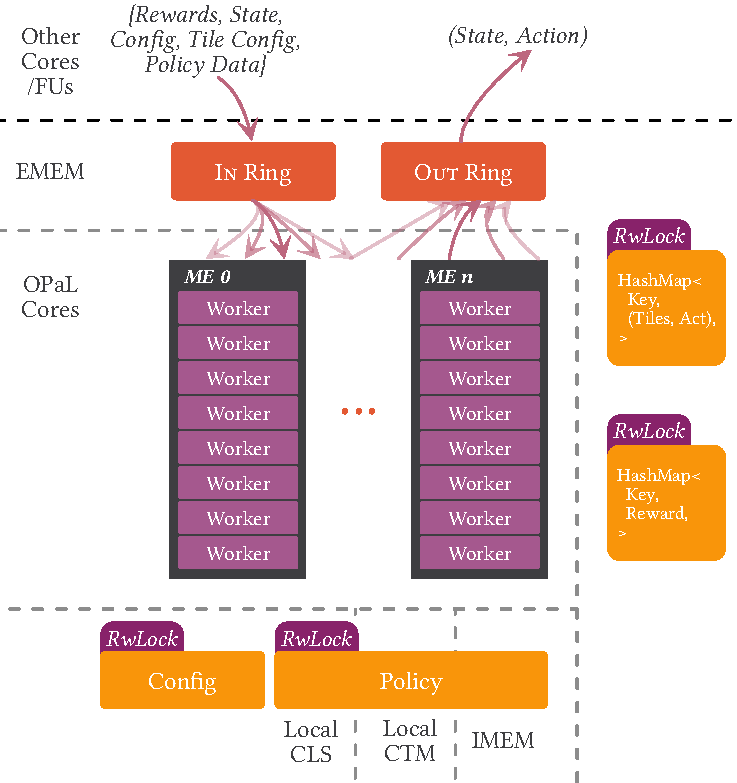
\includegraphics[keepaspectratio, width=0.78\linewidth]{diagrams/opal/ind}
%		\caption{\Indfw{} (offline throughput-optimal). \emph{Workers} independently pull commands from (and push actions to) the environment, locking policy access for updates.\label{fig:single-and-parallel:single}}
%	\end{subfigure}
%
%	\begin{subfigure}{\linewidth}
%		\centering
%		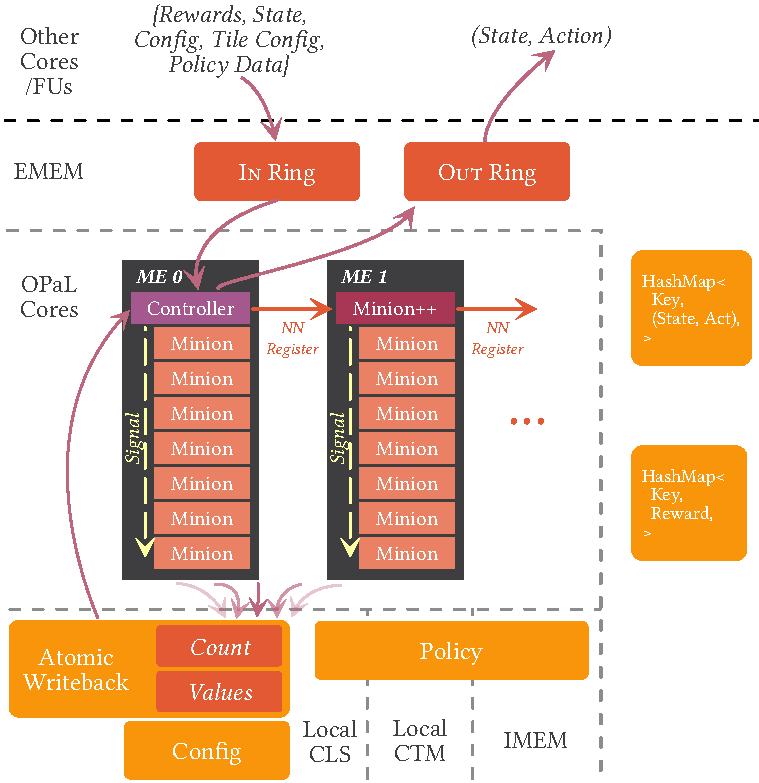
\includegraphics[keepaspectratio, width=0.8\linewidth]{diagrams/opal/coop}
%		\caption{\Coopfw{} (online-optimal). A single \emph{controller} delegates RL computation and updates to many \emph{minion} threads, who operate on independent subtasks.\label{fig:single-and-parallel:parallel}}
%	\end{subfigure}
%	\caption{\approachshort{}'s compute strategies scale to fit device capacity according to either latency or throughput needs.\label{fig:single-and-parallel}}
%\end{figure}

%?? reduce below and make take-homes more generic if possible

\paragraph{Broadcasting}
\approachshort{}'s task broadcast implementation exploits the locality of cores in the \gls{acr:nfp}.
Consider \cref{tab:nfp-ipc-costs}: island-local \gls{acr:ipc} is considerably cheaper than the more generic methods we use for, e.g., the \inring{} and \outring{} rings.
The lowest-latency mechanism here, \emph{next-neighbour registers}, allow for extremely quick communication between \emph{adjacent} \glspl{acr:me}, e.g., 0$\rightarrow$1$\rightarrow$2..., but their use limits us to a chain-forwarding approach.
This remains, however, a net gain over arbitrary messaging via reflector registers in the absence of an actual broadcast bus.
Consider the situation where 4 \glspl{acr:me} are in use, thus the \emph{controller} thread must notify 3 \emph{minion++} contexts.
In a chain forwarding scenario, \glspl{acr:me} 1 and 2 receive commands sooner ($t=$~\qtylist{20; 40}{\nano\second}) than \gls{acr:me} 3---and thus, all their contexts may start work sooner.
Even assuming that all reflector writes can be sent in parallel, their use would enforce that all threads start at $t=$~\qty{60}{\nano\second}.
Reflector register \gls{acr:ipc} does remain a useful option for skipping ahead into chains of larger than 4 \glspl{acr:me}, though these larger islands may only be used when an administrator is willing to replace one or more P4 pipelines.
Inside of an \gls{acr:me}, recall that all contexts share LMEM and a large register file.
As such, work is passed out by copying the received message into a shared register region and simply notifying all other local contexts to awaken.

\paragraph{Aggregation}
Each context writes back to a single shared block of memory in CLS, performing atomic adds to a shared preference list and acknowledgement counter as required by the \emph{Parsa} algorithm.
The controller thread checks these whenever it is notified of task completion by a hardware signal fired after the acknowledgement counter is aggregated.
This is essential for aggregation compared to the use of bounded message buffers, which caused significant head-of-line blocking in earlier implementations.

%?? And NOW discuss bargain-bucket \gls{acr:simd}!
It is worth noting that CLS supports only \qtylist{32;64}{\bit} atomic arithmetic, and the native \gls{acr:nfp} register width is \qty{32}{\bit}.
As a result, lower bit depth tile representations (\qtylist{8;16}{\bit}) ultimately resolve to \qty{32}{\bit} atomic arithmetic.
Is there a way to take advantage of this to gain additional throughput for these tile widths?
That is, to find a bit-packing strategy which enables multiple additions to be performed in a single atomic operation as a makeshift form of \gls{acr:simd}?
While this is doable, the main issue is that additions are performed on signed data in effectively an unsigned way, as the carry between arbitrary bit pairs cannot be disabled.
\emph{Unsigned} overflows are a common occurrence when operating on signed data in this manner\sidenote{Recall that \mintinline{rust}{-1i8}$\rightarrow$\mintinline{rust}{0i8} is also \mintinline{rust}{0xffu8}$\rightarrow$\mintinline{rust}{0x00u8}. As we can reasonably expect individual tile preferences for each action to oscillate between positive and negative, each sign change will trigger an unsigned overflow.}: na\"{i}ve packing will cause the sign changes of adjacent computations to `bleed into' adjacent fields.
In the non-atomic case a single packing bit suffices between any pair of values, all of which may be masked out in a single \gls{acr:alu} operation.
In the atomic case, $n$~\unit{\bit} padding fields allow at most $2^n-1$ additions from separate tasks without clearing.
Having \num{136} tasks and \num{31} workers we require at least \qty{8}{\bit} padding to elide all atomic clears, or \qty{5}{\bit} if every addition is followed by a test-clear operation on all padding bits.
\Cref{fig:bb-simd} shows the packing layouts in a \qty{64}{\bit} field which maximise theoretical throughput---\qtyrange{4}{5}{\times} for \qty{8}{\bit} and \qty{3}{\times} for \qty{16}{\bit}.
%The effectiveness of this scheme is examined in \cref{f}.
Unfortunately, as related in \cref{sec:opal-evaluation}, this adds a consistent \qty{10}{\percent} latency overhead to tile coded inference due to the additional non-atomic \gls{acr:alu} operations needed to pack the input data.
This can be useful on other platforms where atomic operations are much more expensive, or \gls{acr:alu} use is cheaper.

\begin{figure}
	\centering
	\begin{bytefield}{32}
		\bitheader{0,7,8,15,16,23,24,31} \\
		\bitbox{16}[]{\mintinline{rust}{i16}$_0$} &
		\bitbox{8}[bgcolor=bitscratch]{} &
		\bitbox{8}[]{\mintinline{rust}{i16}$_1$} \\
		\bitbox{8}[]{...\mintinline{rust}{i16}$_1$} &
		\bitbox{8}[bgcolor=bitscratch]{} &
		\bitbox{16}[]{\mintinline{rust}{i16}$_2$}
	\end{bytefield}

	\vspace{1em}
	\begin{bytefield}{32}
		\bitheader{0,7,8,15,16,23,24,31} \\
		\bitbox{8}[bgcolor=bitscratch]{} &
		\bitbox{8}[]{\mintinline{rust}{i8}$_0$} &
		\bitbox{8}[bgcolor=bitscratch]{} &
		\bitbox{8}[]{\mintinline{rust}{i8}$_1$} \\
		\bitbox{8}[bgcolor=bitscratch]{} &
		\bitbox{8}[]{\mintinline{rust}{i8}$_2$} &
		\bitbox{8}[bgcolor=bitscratch]{} &
		\bitbox{8}[]{\mintinline{rust}{i8}$_3$}
	\end{bytefield}

	\vspace{1em}
	\begin{bytefield}{32}
		\bitheader{0,5,6,7,8,10,11,15,16,18,19,23,24,29,30,31} \\
		\bitbox{8}[]{\mintinline{rust}{i8}$_0$} &
		\bitbox{8}[bgcolor=bitscratch]{} &
		\bitbox{8}[]{\mintinline{rust}{i8}$_1$} &
		\bitbox{6}[bgcolor=bitscratch]{} &
		\bitbox{2}[]{\mintinline{rust}{i8}$_2$} \\
		\bitbox{6}[]{...\mintinline{rust}{i8}$_2$} &
		\bitbox{5}[bgcolor=bitscratch]{} &
		\bitbox{8}[]{\mintinline{rust}{i8}$_3$} &
		\bitbox{5}[bgcolor=bitscratch]{} &
		\bitbox{8}[]{\mintinline{rust}{i8}$_4$}
	\end{bytefield}
	\caption[Bit-packing layouts for emulated SIMD addition using atomics.]{Bit-packing layouts within a big-endian \qty{64}{\bit} integer required to emulate \gls{acr:simd} addition using atomics. Packing requirements prevent the ideal \qtylist{4;8}{\times} throughput gain for \qtylist{16;8}{\bit} data we'd expect from hardware \gls{acr:simd}. These layouts achieve \qtylist{3;4;5}{\times} \gls{acr:alu} throughput, where the latter \mintinline{rust}{i8} layout requires an explicit atomic clear after every addition. These maximise the count of byte-aligned data, though this cannot be guaranteed as we require at least $\log_2(\mathit{workers})$ bits of internal padding.\label{fig:bb-simd}}
\end{figure}

\paragraph{Initialisation}
Any aggregation step requires us to first know the total number of workers.
This can vary under the number of \glspl{acr:me} running \approachshort{}, the number of contexts assigned to each if CLS/CTM usage is required for another application, and because future designs may also introduce workers on other islands.
This allocation of cores or chip area is set ahead of time by a framework or system administrator, but to enable greater runtime flexibility \approachshort{}-\Coopfw{} agents enumerate themselves at runtime, during initialisation.
To determine this, at startup the controller thread writes its own number of contexts into the first preference list entry, and passes on a message to its next neighbour.
Each \emph{minion++} then adds to this its own number of contexts, and forwards the message to the next \gls{acr:me} in turn.
The last \emph{minion++} worker then increments the acknowledgement counter by 1.
This count is then propagated back out to all contexts, acknowledged and awaited (for, e.g., local workset computation).

\paragraph{Parallels in other platforms}
On other \gls{acr:soc} SmartNICs, we assume that similar \gls{acr:mpmc} communication channels and direct core-to-core messaging are possible under similar constraints, but note that this could be accelerated further by a true broadcast primitive.
If the platform includes true message broadcast then implementation is simple.
More specialised targets such as \gls{acr:fpga}-based solutions may include an explicit bus between the controller and all minion \glspl{acr:fu} to provide this in the most efficient manner possible.
On NetFPGA, the writeback step can make use of native-width adders matching the tile data format, providing hardware \gls{acr:simd} acceleration as required.

%On-chip local messages cost us just $\sim$\qty{20}{\nano\second} latency per relayed message
%
%In earlier designs we had experimented with bounded buffers as in \cref{sec:agent-environment-communication} for this, modified to be located solely in CLS memory, dedicating the master thread to result aggregation.
%We found that this created a performance bottleneck at this final stage, causing significant head-of-line blocking for each of the workers.
%Similarly, our next neighbour work notification scheme ($\sim$\qty{20}{\nano\second} latency per relayed message) was examined against \emph{reflector} and \emph{work queue} IPC mechanisms (\qtylist{58;126}{\nano\second} per messaged core).
%These slower messages can be used in theory to skip ahead into longer ME chains.

%Our implementation exploits the locality of threads, cores, and their parent islands in the NFP architecture.
%Policy compute/update tasks and configuration updates are passed between cores using these direct \emph{next neighbour} registers, signalling all child threads in response.
%Each task performs atomic adds to a shared preference list, and atomically increments an acknowledgement counter to be periodically checked by the master thread, implementing the wait-free \emph{ParSa} algorithm we introduce (\cref{alg:parsa}).

%In earlier designs we had experimented with bounded buffers as in \cref{sec:agent-environment-communication} for this, modified to be located solely in CLS memory, dedicating the master thread to result aggregation.
%We found that this created a performance bottleneck at this final stage, causing significant head-of-line blocking for each of the workers.
%Similarly, our next neighbour work notification scheme ($\sim$\qty{20}{\nano\second} latency per relayed message) was examined against \emph{reflector} and \emph{work queue} IPC mechanisms (\qtylist{58;126}{\nano\second} per messaged core).
%These slower messages can be used in theory to skip ahead into longer ME chains.

\subsection{Reconfigurability}\label{sec:reconfigurability}
\approachshort{} allows policy design and learning parameters to be changed at runtime using at most two control packets.
For instance, design changes are useful at the end of learning (moving from online to offline), or when trying to train a new policy for another problem from the same vantage point.
Parameter changes are useful when an online agent must become more (or less) adaptive to new data (i.e., after detecting a changepoint in traffic).
This extends to policy data, which may be imported from a pre-trained model via such packets and exported via \gls{acr:pcie} to the host machine.
Some aspects must be chosen at compile time; bit depth, parallelism strategy via \Coopfw/\Indfw, and maximum policy, tiling, or state sizes---these govern core operation or pre-allocated memory.
Choosing a bit depth of \qtylist[list-pair-separator = { or }]{16;8}{\bit} halves/quarters policy memory costs, allowing more complex problems to be modelled using more dimensions or fine-grained tiles.

In this implementation, configuration packets are carried over \gls{acr:udp} and signalled to the P4 parser using a reserved pool 2 \gls{acr:dscp}~\parencite{rfc2474} value, similarly to \textcite{DBLP:conf/isca/LiLYCSH19}.
While this mainly automates parser generation, it also allows for configuration to be received from only trusted hosts (over the dataplane if needed) via P4 rules.
The control packet generation library and evaluation frameworks which build upon it are written in Rust.

%?? Need protocol diagrams?

%Runtime reconfiguration and interaction occur via the control and/or dataplane: the ease of use of the P4 pipeline's match-action tables and custom protocol parsers, combined with the dedicated input pipe to the NIC's controller (the host machine), allow these to be cleanly separated or combined as needed.
%Bit depth of quantised measurements/preferences, maximum policy sizes, and parallelisation strategy may be configured at compile time.

\subsection{Work allocation}\label{sec:work-allocation}
\begin{algorithm}
	\caption{Task scheduling for ParSa\label{alg:parsa-schedule}}
	\tcc{Assume we have a list \emph{ME\_CTXS}, which contains one entry for each included \gls{acr:me} counting the number of its usable contexts, totalling \emph{N\_CTXS}. Also, assume we know the average cost of a task in each memory region, \emph{MEM\_COSTS}.}
	\SetKw{Let}{let}
	\SetKw{Enum}{enum}
	\SetKw{Struct}{struct}
	\SetKw{In}{in}
	\SetKw{Await}{await}
	\SetKw{Return}{return}
	\SetKw{Forkw}{for}
	\SetKw{Const}{const}
	\Struct Cost \{ \emph{cost}, \emph{n\_items}, \emph{max\_items} \}\;
	\SetKwProg{sched}{Function \emph{Schedule}}{}{end}
	\sched{work\_items}{
		\Let \emph{out} = vec![vec![]; \emph{N\_CTXS}]\;
		\Let \emph{alloc\_sz} = \emph{work\_items}.len() $\div$ \emph{N\_CTXS}\;
		\Let \emph{alloc\_spill} = \emph{work\_items}.len() \% \emph{N\_CTXS}\;
		\Let \emph{me\_costs} = [Cost \{ 0, 0, 0 \}; \emph{ME\_CTXS}.len()]\;
		\Let \emph{ctx\_costs} = [Cost \{ 0, 0, \emph{alloc\_sz} \}; \emph{ME\_CTXS}.len()]\;
		\ForAll{ctx \In ctx\_costs[..alloc\_spill]}{
			\emph{ctx.max\_items} += 1\;
		}
		\ForAll{ctx \In ctx\_costs}{
			\Let \emph{penalise\_early\_ctx} = \emph{ME\_CTXS}[me\_id(\emph{ctx})] - \emph{local\_ctx\_id}(\emph{ctx}) - 1\;
			\emph{me\_costs}[me\_id(\emph{ctx})]\emph{.max\_items} += \emph{ctx.max\_items}\;
			\emph{ctx.cost} = \emph{penalise\_early\_ctx}\;
			\emph{me\_costs}[me\_id(\emph{ctx})]\emph{.cost} += \emph{ctx.cost}\;
		}
		\tcp{Sort MEs by cost / \emph{ME\_CTXS}[\emph{me}], breaking ties on largest id.}
		\Let \emph{me\_heap} = min\_heap(\emph{me\_costs})\;
		\tcp{Sort CTXs by cost, breaking ties on smallest id.}
		\Let \emph{ctx\_heaps} = [min\_heap(\emph{ctx\_costs}[\emph{first\_ctx}(\emph{me})..\emph{ME\_CTXS}[\emph{me}]]) \Forkw \emph{me} \In 0..\emph{ME\_CTXS}.len()]\;
		\ForAll{item \In work\_items.reverse()}{
			\Let \emph{me} = find\_min(\emph{me\_heap})\;
			\Let \emph{ctx} = find\_min(\emph{ctx\_heaps}[\emph{me}])\;
			\emph{me.n\_items} += 1\;
			\emph{ctx.n\_items} += 1\;
			\uIf{me.n\_items $\ge$ me.max\_items}{
				\emph{me\_heap}.remove(\emph{me})\;
			}
			\Else{
				\emph{me.cost} += \emph{MEM\_COSTS}[\emph{item.region}]\;
				\emph{me\_heap}.rebalance()\;
			}
			\uIf{ctx.n\_items $\ge$ ctx.max\_items}{
				\emph{ctx\_heaps}[\emph{me}].remove(\emph{ctx})\;
			}
			\Else{
				\emph{ctx.cost} += \emph{MEM\_COSTS}[\emph{item.region}]\;
				\emph{ctx\_heaps}[\emph{me}].rebalance()\;
			}
			
			\emph{out}[\emph{ctx}].push(\emph{item})\;
		}
		\Return{\emph{out}}
	}
\end{algorithm}

I use a simple first-fit work placement algorithm, \cref{alg:parsa-schedule}, run in \approachshort{}-\Coopfw{} whenever a full configuration is installed.
This places the largest work item into the least loaded minion context of the least loaded \gls{acr:me}, and assigns an equal number of tasks among all \glspl{acr:me} where possible.
Each work item is a separate \emph{tiling} over a list of dimensions, where it can be reasonably assumed that these items are sorted by dimension count---thus, the reversed work list places the most computationally expensive tasks first.
The approximate cost of any work item according to its dimension count and memory location was empirically measured offline and fed back into ther scheduler---a mean \qtylist{5.2;6.2;9.7;11.0}{\micro\second} for bias (0D), CLS (1D), CTM ($\le$2D) and IMEM ($\le$4D) tilings respectively.
Finally, this scheduler weighs the total cost per core based on the number of minion threads available.
This weighting specifically accounts for the controller thread on the first core.
To work around some fairly opaque waking behaviour between contexts on each \gls{acr:me}, I apply a small penalty to minion contexts with a lower internal ID.

Naturally, for $n$ tilings and $m$ threads this procedure is $\mathcal{O}{\left(n\log{m}\right)}$: two find/update min operations into binary heaps per tiling, storing $m/8$ and $\le8$ costs respectively.
As an implementation detail, given that number of \glspl{acr:me} is small we may replace their minheap with a list to reduce the setup overhead (i.e., constant terms) in exchange for worse asymptotic scaling.
This also enables us to compare $\textit{cost}_i \times \textit{ME\_CTXs}\left[\textit{best}\right] \le \textit{cost}_\textit{best} \times \textit{ME\_CTXs}\left[i\right]$ rather than repeatedly apply fixed-point division.
%$\textit{cost}_i \times \textit{ME\_CTXs}\left[\textit{best}\right]$

%?? Redo and fully explain.

%\subsection{Variable Quantisation Bit Depth}
%At compile-time, \approachshort{} can be configured to use \qtylist[list-final-separator = { or }]{32;16;8}{\bit} values in input states and its internal policies.
%Naturally, smaller bit depths reduce the storage required for policies, tiling data, and stored state-action pairs---allowing more complex problems to be modelled using more dimensions or fine-grained policies.
%Through the lens of computational efficiency, reduced bit depth should allows action preference lists to be read using fewer I/O operations (as more values may fit into a single machine word).
%
%We had investigated bit-stuffing several such values into a single word for our atomic writeback mechanism (as the platform offers both \qtylist{32;64
%}{\bit} atomic addition).
%This is analogous to SIMD---through clever use of padding bits---but we found that manipulating tiles into the correct format added \qty{10}{\percent} extra overhead.
%We investigate further performance implications of changing bit depth in the sequel.

%Potential: low-latency train for some specific points, and high throughput for others? Think on the exact note I took...
%
%``can have accel'd offline, train online subset w/ my approach''
%
%THis might mean "do 32-bit online", then downsample to 8-bit policy for high-throughput mode.
%
%Can changes in trained policy be used to transfer to a more complex function approximator elsewhere?

%As is expected of parallel algorithms, efficient division of work, communication, and aggregation add per-task overheads in both the serial and parallel portions.


%\subsection{Targeting other device classes}
%While this design caters to Netronome devices, many aspects have clear analogues in other SmartNICs, such as the NetFPGA SUME.
%For instance, additional off-path functional units can serve as workers, like the floating-point adders used by \textcite{DBLP:conf/isca/LiLYCSH19}.
%Rather than general-purpose IPC, \approachshort{} would be hard-wired between internal workers and to the P4$\rightarrow$NetFPGA~\parencite{DBLP:conf/fpga/IbanezBMZ19} actions that interface with it.
%%Further optimisations arise from this model: a NetFPGA design would be able to replicate and optimise further on this concept of dedicated, low-latency communication between functional units.
%As we show later, using a bit depth below the native word size reduces overall efficiency.
%%This reduces overall efficiency even though considerably fewer reads are made.
%We expect an FPGA design would allow this to match the desired bit depth and enable the SIMD-like optimisations we discuss without creative and costly bit-stuffing.

%While specifics of this design cater to Netronome devices, many aspects have clear analogues in NICs of similar form-factor, such as the NetFPGA SUME platform.
%For instance, other cores can be introduced by designing additional off-path functional units,  like the floating-point adders used by \textcite{DBLP:conf/isca/LiLYCSH19}.
%Rather than general-purpose IPC, \approachshort{} would be hard-wired between internal workers and to the custom actions that interface with it, using the P4$\rightarrow$NetFPGA toolchain to offer granular control over packet and flow selection.
%%Further optimisations arise from this model: a NetFPGA design would be able to replicate and optimise further on this concept of dedicated, low-latency communication between functional units.
%As our later results show, using a bit depth below the native word size forces the compiler to emit excess code to extract and re-align preference values, reducing overall efficiency.
%%This reduces overall efficiency even though considerably fewer reads are made.
%We expect that a more bespoke hardware/FPGA design would allow this to match the desired bit depth and enable SIMD-like optimisations we discuss without creative and costly bit-stuffing.
%
%Bringing \approachshort{} to high-port density devices such as Tofino-powered switches is more difficult.
%As discussed in \cref{sec:motivation}, Tofino ASICs map closely to the P4 PSA, meaning that there are no spare asynchronous general-purpose compute units to place this work on.
%Taking inspiration from real-time programming techniques, a potential solution is to divide RL actions across several received packets (i.e., iteratively computing a portion of the action preference list each time) until any further work would delay outbound transmission.
%This, however, would introduce new issues surrounding concurrent accesses, work splitting, and altered timescales for learning: we leave their treatment and examination to future work.